\documentclass[12pt,a4paper]{article}

\usepackage{buaa_paper}

\schoolname{北京航空航天大学计算机学院}
\title{学位论文开题报告}
\papertitle{神经网络语言模型的性能优化研究}
\specialty{计算机科学与技术}
\studentnumber{SY1506330}
\researcharea{自然语言处理}
\advisor{荣文戈~~副教授}
\author{姜~~楠}
\date{2016 年 12 月 20 号}

\begin{document}

\maketitle

\tableofcontents
\newpage


\section{论文选题的背景与意义}
近年来,随着Web2.0 的兴起,互联网上的数据急剧膨胀。根据国际数据公司(IDC)的统计和预测,2011 年全球网络数据量已经达到1.8ZB,到2020 年,全球数据总量预计还将增长50 倍。大量无标注数据的出现,也让研究人员开始考虑,如何利用算法从这些大规模无标注的文本数据中自动挖掘规律,得到有用的信息。2006年, Hinton 提出的深度学习\cite{hinton2006reducing},为解决这一问题带来了新的思路。在之后的发展中,基于神经网络的表示学习技术开始在各个领域崭露头角。尤其在图像和语音领域的多个任务上,基于表示学习的方法在性能上均超过了传统方法。

近年来,深度学习逐渐在自然语言处理中得到应用. 研究者提出用神经网络(Neural Network, NN) 来训练语言模型并进行了相关探索\cite{DBLP:conf/nips/BengioDV00}. 其中,基于循环神经网络的语言模型建模方法引起了研究者极大的兴趣[3]. 网络通过学习能够将当前词的历史信息存储起来,以词的整个上下文作为依据,来预测下一个词出现的概率,克服了n-gram 语言模型无法利用语句中长距离上下文信息的缺点. 另外,在模型训练的过程中,由于词的历史信息被映射到低维连续空间,语义相似的词被聚类,在语料中出现次数较少的词仍然能够得到很好的训练,不再需要额外的数据平滑技术. 迄今为止,采用(Recurrent Neural Network, RNN)训练的语言模型在模型困惑度(Perplexity, PPL)和识别系统的识别率上都取得了最好的效果[4]. RNN 建模方法虽然表现出极大的优越性,却以牺牲计算复杂度为代价. 若训练大规模的文本语料,则需要花费很长的时间,制约了RNN 语言模型训练效率. 为克服这一不足,文献[5] 提出了多种优化策略来降低网络的计算复杂度,如缩短模型训练周期、减少训练数据集的规模、降低训练词典的大小、减少隐含层的节点数等,这些方法都在一定程度上降低了网络的运算量,提高了模型的训练效率,但同时也牺牲了较多的模型性能. 另外,在网络结构层面上,文献\cite{DBLP:journals/coling/BrownPdLM92} 研究了一种基于分类的循环神经网络(Class-based RNN) 结构,网络的输出层被分解为两部分,增加的一部分称为分类层,从结构上降低了整个网络的计算复杂度,使得模型训练效率有了一定的提升且模型性能没有大的变化. 然而,在大词汇量连续语音识别系统中,采用此结构训练大规模语料语言模型仍需要花费大量时间. 因此,模型训练效率有待进一步优化.

因此探讨研究语言模型的大词表问题,是目前理论应用到实际过程中必须要克服的问题。我们当然可以通过配置高性能服务器来暂时延缓该问题的后果,但是一旦应用到大数据集上,即使是目前最好的CPU或者GPU,仍然需要三五天时间才能训练完善。应此,在保证原有模型的准确率的目的下,如何提高模型的训练速度是我们主要讨论的内容。为此我们讨论了三个不同的方向:一种是通过采样技术(Importance Sampling)来减少必要的训练时间;一种是通过基于分类的多元分类(class-based hierarchical softmax, cHSM)来加速模型; 最后一种是采用基于树模型的多层二元分类模型(tree-based hierarchical softmax, tHSM).

同时,我们还需要针对CPU 和GPU设备分别进行探讨。因为传统的线性运算模型在流行的GPU并行运算方案中并不适用,所欲需要结合不同的运算设备分别讨论可行的方案。

\section{国内外研究现状及发展动态}
基于神经网络的分布表示一般称为词向量、词嵌入(word embedding)或分布式表示(distributed representation)[116]。神经网络词向量表示技术通过神经网络技术对上下文,以及上下文与目标词之间的关系进行建模。由于神经网络较为灵活,这类方法的最大优势在于可以表示复杂的上下文。在前面基于矩阵的分布表示方法中,最常用的上下文是词。如果使用包含词序信息的n-gram 作为上下文,当n 增加时,n-gram 的总数会呈指数级增长,此时会遇到维数灾难问题。而神经网络在表示n-gram 时,可以通过一些组合方式对n 个词进行组合,参数个数仅以线性速度增长。有了这一优势,神经网络模型可以对更复杂的上下文进行建模,在词向量中包含更丰富的语义信息。神经网络模型主要包括: 传统前向传递神经网络(Feed Forward Neural Network, FFNN)、循环神经网络(Recurrent Neural Network,RNN)建模方案。

另外针对大词表问题,主要可以分为以下两种策略:基于类别的多元分类模型(class-based hierarchical softmax, cHSM)和基于二叉树的二元分类模型(class-based hierarchical softmax, tHSM),我们分别在下面详细讨论和介绍。
\subsection{语言模型简介}
语言模型可以对一段文本的概率进行估计,对信息检索、机器翻译、语音识别等任务有着重要的作用。
形式化讲,统计语言模型的作用是为一个长度为m 的字符串确定一个概率分布$P(w_1;w_2;\cdots;w_m)$,表示其存在的可能性,其中$w_1$ 到$w_m$ 依次表示这段文
本中的各个词。一般在实际求解过程中,通常采用下式计算其概率值:
\begin{equation}
\label{equ:lm}
\begin{split}
P(w_1;w_2; \cdots;w_m) &= P(w_1) P(w_2|w_1) P(w_3|w_1;w_2)\cdots P(w_i | w_1;w_2;\cdots;w_{i-1}) \\
&\cdots P(w_m | w_1;w_2;\cdots;w_{m-1})
\end{split}
\end{equation}
在实践中,如果文本的长度较长,公式\ref{equ:lm}右部$\cdots P(w_m | w_1;w_2;\cdots;w_{m-1}) $ 的估算会非常困难。因此,研究者们提出使用一个简化模型:n 元模型(n-gram model)。在n 元模型中估算条件概率时,距离大于等于n 的上文词会被忽略,也就是对上述条件概率做了以下近似:
\begin{equation}
\label{equ:approx}
P(w_i | w_1;w_2;\cdots;w_{i-1})  \approx P(w_i | w_{i-(n-1)};\cdots;w_{i-1})
\end{equation}
当$n = 1$ 时又称一元模型(unigram model),公式\ref{equ:approx} 右部会退化成$P(w_i)$,此时,整个句子的概率为:$P(w_1;w_2; \cdots;wm) = P(w_1)P(w_2) \cdots P(w_m)$。从式中可以知道,一元语言模型中,文本的概率为其中各词概率的乘积。也就是说,模型假设了各个词之间都是相互独立的,文本中的词序信息完全丢失。因此,该模型虽然估算方便,但性能有限。

当n = 2 时又称二元模型(bigram model),将n 代入公式\ref{equ:approx} 中,右部为P$(w_i|w_{i-1})$。常用的还有n = 3 时的三元模型(trigram model),使用$P(w_i |w_{i-2};w_{i-1})$ 作为近似。这些方法均可以保留一定的词序信息。

\subsection{上下文信息的建模策略}
上下文信息建模策略主要的思路包括: 传统前向传递神经网络(Feed Forward Neural Network, FFNN)、循环神经网络(Recurrent Neural Network,RNN)建模方案。 以下我们一一探讨。

Xu 等人在2000 年首次尝试使用神经网络求解二元语言模型[124]。2001年,Bengio 等人正式提出神经网络语言模型(Neural Network Language Model ,NNLM)[6, 7]。该模型在学习语言模型的同时,也得到了词向量。NNLM 同样也是对n 元语言模型进行建模,估算$P(w_i | w_{i-(n-1)}; \cdots ;w_{i-1})$的值。但与传统方法不同的是,NNLM 不通过计数的方法对n 元条件概率进行估计,而是直接通过一个神经网络结构,对其进行建模求解。图\ref{fig:ffnn} 展示了NNLM 的基本结构。

\begin{figure}
  \centering
  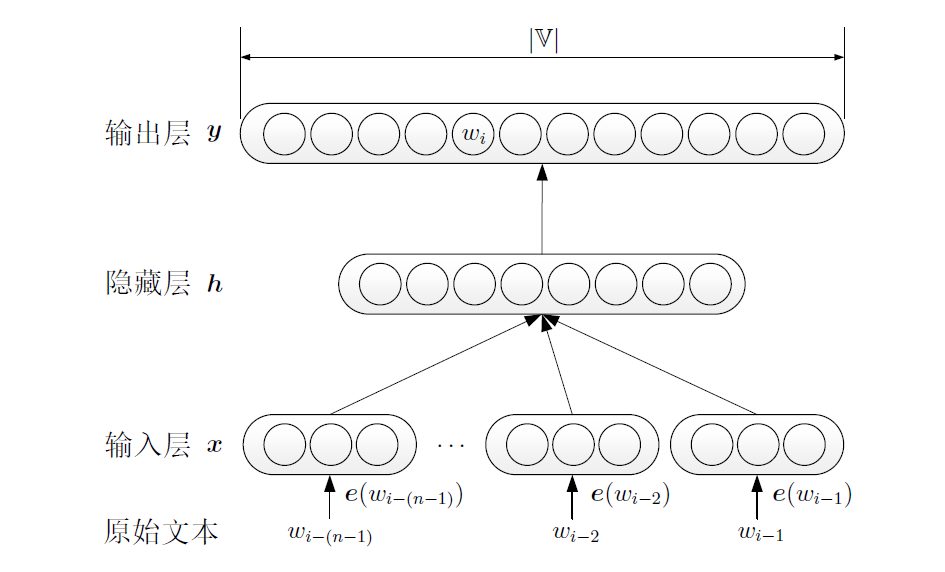
\includegraphics[width=0.8\linewidth]{./figures/ffnn.png}
  \caption{神经网络语言模型(NNLM)模型结构图}\label{fig:ffnn}
\end{figure}

Mikolov等人提出的循环神经网络语言模型(Recurrent Neural Network based Language Model,RNNLM)则直接对$P(w_i | w_1;w_2;\cdots;w_{i-1}) $ 进行建模,而不使用公式\ref{equ:approx}对其进行简化[72, 74]。因此,RNNLM 可以利用所有的上文信息,预测下一个词,其模型结构如图\ref{fig:rnnlm} 所示。
\begin{figure}
  \centering
  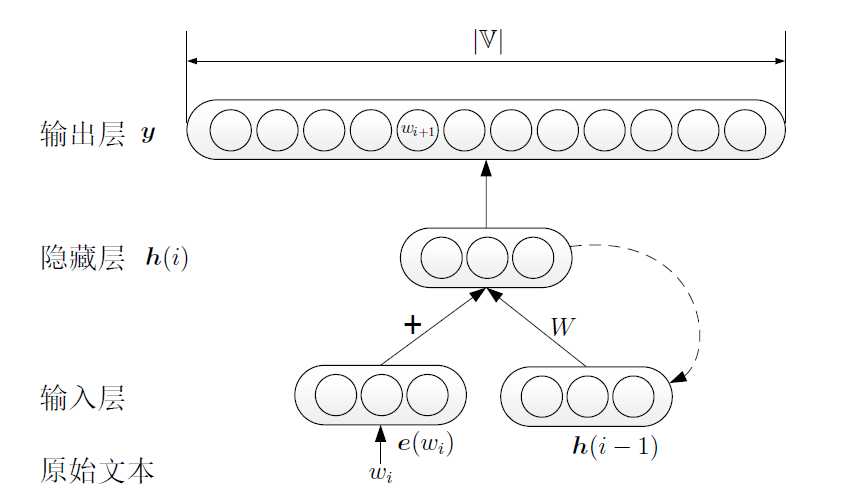
\includegraphics[width=0.85\linewidth]{./figures/rnnlm.png}
  \caption{循环神经网络语言模型(RNNLM)模型结构图}\label{fig:rnnlm}
\end{figure}

RNNLM 的核心在于其隐藏层的算法:
\begin{equation}
\label{equ:rnn}
h(i) =\phi(e(w_i) +Wh(i -1))
\end{equation}
其中,$\phi$非线性激活函数。但与NNLM 不同,RNNLM 并不采用n 元近似,而是使用迭代的方式直接对所有上文进行建模。在公式\ref{equ:rnn} 中,h(i) 表示文本中第$i$ 个词$w_i$ 所对应的隐藏层,该隐藏层由当前词的词向量$e(wi)$ 以及上一个词对应的隐藏层$h(i -1)$ 结合得到。

\subsection{多元分类模型}
传统的多元分类模型(Softmax):
\begin{equation}\label{equ:softmax}
  \hat y_i=\frac{\exp(o_i)}{\sum_j \exp(o_j)}
\end{equation}
其中由于分母是正则项,一旦词表扩大,每次迭代更新都需要计算这一项,是主要的问题所在,所以本课题拟在主要解决该问题所导致的计算费时的问题,在保证计算精度不下降的情况下,提高模型的训练速度。目前主要的策略分为: 基于类别的多元分类模型(class-based hierarchical softmax, cHSM)和基于二叉树的二元分类模型(class-based hierarchical softmax, tHSM).

假设语料中的每一个词样本属于且只属于一个类,在此基础上计算词样本在语料中的分布时,可以先计算类的概率分布,然后在所属类上计算当前词的概率分布,于是可将式(3)转化为

\begin{equation}\label{equ:class}
  p(w_i|h_i) = p(c(t)|h(t))p(w_i|c(t))
\end{equation}
此时,训练一个词样本的计算复杂度正比于:$O =HC$. 式中,C 为语料中所有词的分类数,可根据语料中词的词频进行划分. 当C 取1 或取词典大小V 时,此结构等同于标准的RNN 结构. 由于$C \ll V$,通过图1 结构训练的softmax 降低了计算复杂度.

Mikolov曾提出使用基于二叉树的层级softmax模型来加速的训练方案,加速比能达到理论的最大速度,但是当时提出的背景是基于CPU构建的,如今越来越多的算法随着应用领域的推广,需要在并行度更高的GPU上进行计算,因此基于GPU进行建模的tHSM尚未被研究提及,需要后人研讨。


\section{论文的研究内容及拟采取的技术方案}
\subsection{对上下文信息建模策略}
依照上章节的分析,本章节主要介绍我们实验中所要涉及的模型,主要分为: 长短记忆网络(Long shrot-term memory, LSTM)和门限记忆节点(Gated Recurrent Unit,GRU)。

LSTM的计算公式定于如下:
\begin{itemize}
\item 输入门:控制输入的信息流:
$$i_t=\sigma(W^i x_t+U^i h_{t-1}+b^i)$$
\item  遗忘门:控制信息遗忘的速度:
$$f_t=\sigma(W^f x_t+U^f h_{t-1}+b^f)$$
\item  信息更新值:
$$g_t=\phi(W^g x_t+U^g h_{t-1}+b^g)$$
\item  输出门:
$$o_t=\sigma(W_o x_t+U^o h^{t-1}+b^o)$$
\item  中间状态更新:
$$s_t=g_t\cdot i_t+s_{t-1}\cdot f_t$$
\item  隐藏层的输出值:
$$h_t=s_t\cdot \phi(o_t)$$
\end{itemize}
其中$\cdot$ 代表"element-wise matrix multiplication"(对应元素相乘),$\phi(x)=\tanh(x),\sigma(x)=sigmoid(x)$
$$\phi(x)=\frac{e^x-e^{-x}}{e^x+e^{-x}},\sigma(x)=\frac{1}{1+e^{-x}}$$

GRU和lstm的计算公式很相似,具体定义如下:
\begin{itemize}
\item 更新门$z_t$: 定义保存多少以前的信息。

\[z_t = \sigma ( W^z x_t+ U^z h_{t-1}  )\]

\item 重置门$r_t$: 决定保留多少输入信息.

\[r_t = \sigma(W^r x_t  + U^r h_{t-1}  )\]

\item 节点内部更新值$\tilde h_t $:
 \[\tilde h_t  = \tanh (W^h x_t  + U^h(h_{t-1} \odot r_t) )\]

\item 隐藏层输出值$h_t$:
\[h_t = (1-z_t)\odot \tilde h_t  + z_t \odot h_{t-1}\]
\end{itemize}

\subsection{对多元分类模型的建模}
大词表问题,主要是对softmax如何建模的问题。在本课题中,我们探讨cHSM和tHSM两种不同的方案所带来的影响和优劣。
\subsection{单词聚类的策略}
当我们使用多层分类模型的时候,我们就需要将单词按照模型的架构进行划分。其中对于cHSM模型,我们有以下策略可以使用:1) 基于词频划分类别 2) 基于2-gram 的布朗聚类(brown clustering) 进行划分.3)按照word-embedding 的词向量信息进行聚类。另外,我们还需要注意的是,各个类别可以包含不同的数量的单词,也可以包含数量相同的单词。对于后者,我们考虑的划分模型就是基于交换算法(Exchange Algorithm), 以此来保证获得近似的最优解。

\section{关键技术或技术路线}

1) 数学背景和理论背景。 尽管本实验题目定义范围比较小,但是我们也需要很好的数学理论知识,包括:矩阵论,概率论。还有,我们还需要极强的阅读外文文献知识和编码实现能力,都是不可或缺的基本要求。矩阵在许多学科领域中都有应用,在很多时候,除了需要知道矩阵的理论性质以外,还需要计算矩阵的数值。为了矩阵的计算能够足够精确与快捷,数值线性代数中专门有研究矩阵的数值计算方法[40]。与其它的数值计算一样,矩阵的数值计算注重的主要也是算法的复杂度和数值稳定性。矩阵的数值计算可以使用直接计算,也可以用迭代算法,例如在计算方块矩阵的特征值时,可以从一个非零向量$x_0$开始,通过特定迭代方法得到一个逼近某个特征向量的向量序列[41]。而概率论,作为统计学的数学基础,概率论对诸多涉及大量数据定量分析的人类活动极为重要[3],概率论的方法同样适用于其他方面,例如是对只知道系统部分状态的复杂系统的描述——统计力学,而二十世纪物理学的重大发现是以量子力学所描述的原子尺度上物理现象的概率本质[4]。

2) 基于theano框架的建模方案。因为基于 python 的深度学习库比较完善,适合建模。 本实验拟采用 theano 的建模语言,来帮助我们快速建模和调参。Theano是在BSD许可证下发布的一个开源项目,是由LISA集团(现MILA)在加拿大魁北克的蒙特利尔大学(Yoshua Bengio主场)开发。它是用一个希腊数学家的名字命名的。Python的核心Theano是一个数学表达式的编译器。它知道如何获取你的结构,并使之成为一个使用numpy、高效本地库的非常高效的代码,如BLAS和本地代码(C++),在CPU或GPU上尽可能快地运行。它巧妙的采用一系列代码优化从硬件中攫取尽可能多的性能。如果你对代码中的数学优化的基本事实感兴趣,看看这个有趣的名单。Theano表达式的实际语法是象征性的,可以推送给初学者用于一般软件开发。具体来说,表达式是在抽象的意义上定义,编译和后期是用来进行计算。它是为深度学习中处理大型神经网络算法所需的计算而专门设计的。它是这类库的首创之一(发展始于2007年),被认为是深度学习研究和开发的行业标准。

3) 同时本实验也需要对linux的bash脚本有一定的熟悉,以方便将模型的数据结果正确的统计和运行模型的开发环境配置。

4) 试验结果图表统计和绘制.本实验的结果需要精良的语言来控制,而R语言的ggplot2框架就很适合我们的试验结果图表的绘制工作。

5) 基于GPU的cuda的模型优化也是我们需要考虑的问题之一。 CUDA(Compute Unified Device Architecture,统一计算架构[1])是由NVIDIA所推出的一種整合技術,是該公司对于GPGPU的正式名稱。透过这个技术,使用者可利用NVIDIA的GeForce 8以後的GPU和較新的Quadro GPU进行计算。亦是首次可以利用GPU作為C-编译器的开发环境。NVIDIA行銷的時候[2],往往將编译器与架构混合推廣,造成混乱。实际上,CUDA可以相容OpenCL或者自家的C-编译器。无论是CUDA C-語言或是OpenCL,指令最終都會被驱动程序轉換成PTX代码,交由显示核心計算。

在GPUs(GPGPU)上使用圖形APIs进行传统通用計算,CUDA技术有下列几個优点:
\begin{itemize}
  \item 分散读取——代码可以从内存的任意位址读取
  \item 统一虚拟内存(CUDA 6)
  \item 共用内存——CUDA公开一個快速的共用存储区域(每个处理器48K),使之在多个进程之間共用。其作为一個用戶管理的快取内存,比使用纹理查找可以得到更大的有效频宽。
  \item 与GPU之間更快的下载与回读
  \item 全面支持整型位与操作,包括整型纹理查找
\end{itemize}



限制
\begin{itemize}
  \item CUDA不支持完整的C语言标准。它在C++编译器上運行主機代码時,會使一些在C中合法(但在C++中不合法)的代碼無法編譯。
  \item 不支持紋理渲染(CUDA 3.2及以後版本通過在CUDA陣列中引入“表面寫操作”——底層的不透明数据结构——來进行处理)
  \item 受系统主线的频宽和延遲的影響,主機與設備記憶體之間資料複製可能會導致性能下降(通過過GPU的DMA引擎處理,非同步記憶體傳輸可在一定範圍內緩解此現象)
  \item 当執行緒總數為數千時,执行程序按至少32個一組來運行才能獲得最佳效果。如果每組中的32個進程使用相同的執行路徑,則程式分支不會顯著影響效果;在處理本質上不同的任務時,SIMD執行模型將成為一個瓶頸(如在光線追蹤演算法中遍歷一個空間分割的資料結構)
  \item 与OpenCL不同,只有NVIDIA的GPUs支援CUDA技術
  \item 由于编译器需要使用优化技术來利用有限的资源,即使合法的C/C++有時候也會被標記並中止编译
  \item CUDA(計算能力1.x)使用一個不包含回槊、函数指標的C語言子集,外加一些簡單的扩展。而單個進程必須運行在多個不相交的記憶體空間上,這與其它C語言運行環境不同。
  \item CUDA(計算能力2.x)允许C++类功能的子集,如成員函數可以不是虛擬的(這個限制將在以後的某個版本中移除)[参见《CUDA C程式設計指南3.1》-附錄D.6]
  \item 双精度浮点(CUDA计算能力1.3及以上)与IEEE754標準有所差異:倒数、除法、平方根僅支持舍入到最近的偶數。单精度中不支持反常值(denormal)及sNaN(signaling NaN);只支持两种IEEE舍入模式(舍位与舍入到最近的偶数),這些在每条指令的基楚上指定,而非控制字码;除法/平方根的精度比单精度略低。
\end{itemize}

\section{论文研究计划}
\begin{itemize}
  \item 2016年12月 $\sim$ 2017年1月: 整理资料,学习研究语言模型的领域知识;
  \item 2017年2月$\sim$ 2017年4月: 研究学习深度学习模型的知识, 特别是循环神经网络的建模过程;
  \item 2017年5月$\sim$2017年7月: 调研并实现解决大词表问题的主要手段, 并实现基本代码框架;
  \item 2015年8月$\sim$2015年10月: 实验验证与完善;
  \item 2015年11月$\sim$2015年12月:资料整理和论文撰写.
\end{itemize}

\newpage
\addcontentsline{toc}{section}{主要参考文献}
\bibliography{bibs}

\end{document}
